\documentclass{article}
\usepackage[utf8x]{inputenc}
\usepackage{amsmath}
\usepackage{amsfonts}
\usepackage{amssymb}
\usepackage[margin=2cm, top=1cm, bottom=1.5cm]{geometry}
\usepackage{multicol}
\usepackage{graphicx}
\usepackage{calc}
% \usepackage{slashbox}
\usepackage{bbold}
\usepackage{array}
\usepackage{minted}
\usepackage{alltt}
\usepackage{pstricks-add}
\usepackage{pstricks}
\usepackage{hyperref}
\usepackage{tabularx}
\usepackage{subcaption}
%\newcolumntype{Y}{>{\centering\arraybackslash}X}

\usepackage[inkscapeformat=png]{svg}
\usepackage{caption}
\usepackage{pdfpages}


% Packages pour la mise en page et la personnalisation de la table des matières
\usepackage{tocloft}    % Permet de personnaliser la table des matières
\usepackage{titlesec}   % Permet de personnaliser les titres des sections
\usepackage{lmodern}    % Améliore la police de base
\usepackage{setspace}   % Pour gérer les espaces dans le document

% Personnalisation de la table des matières
\renewcommand{\cftsecfont}{\large\bfseries}  % Sections en gras et en plus grand
\renewcommand{\cftsecpagefont}{\large\bfseries}  % Numéros de page en gras
\renewcommand{\cftsubsecfont}{\normalsize\itshape}  % Sous-sections en italique
\renewcommand{\cftsubsubsecfont}{\normalsize\itshape}  % Soussous-sections en italique
\renewcommand{\cftsubsecpagefont}{\normalsize\itshape}  % Numéros de sous-sections en italique
\renewcommand{\cftsubsubsecpagefont}{\normalsize\itshape}  % Numéros de soussous-sections en italique
\renewcommand{\contentsname}{} % Enlever le "Contents"
\setlength{\cftbeforesecskip}{10pt}  % Espacement avant chaque section



\usemintedstyle{tango}
\renewcommand{\thesection}{\Roman{section}}

\begin{document}

\begin{titlepage}

\newcommand{\HRule}{\rule{\linewidth}{0.5mm}}
\center 


\begin{figure}
    \centering
    
\includegraphics[width=0.5\linewidth]{outputs/title_page/ssd_logo_couleur_noir-300x103.png}
\end{figure}



\textsc{\Large Master 2 Statistiques et Sciences des Données }\\[1cm] % Major heading such as course name
\HRule \\[0.4cm]
{ \huge \bfseries Rapport de TP :\\[0.6cm] Support Vector Machines (SVM) }\\[0.4cm]
\HRule \\[1.5cm]
\begin{center}
\begin{Large}
BOULAND Guillaume \\

\end{Large}
\end{center}
    
\vfill
\begin{center}
\includegraphics[width=0.1\linewidth]{outputs/title_page/Logo_université_montpellier.png}\vspace{0.5cm}\\
\begin{Large} Année 2024 - 2025 \\
\end{Large}
\end{center}

\end{titlepage}
\newpage

% Crée la table des matières avec un titre personnalisé
\begin{center}
    {\LARGE\bfseries Table des matières}
\end{center}
\vspace{1cm}  % Espace entre le titre et la table des matières
\tableofcontents
\vspace{1cm} 
\newpage

Le code complet est disponible sur notre \href{https://github.com/guibouland/TP3_AP_SVM}{Github} dans le fichier \texttt{svm\_script.py}, dans le dossier \texttt{src}. Il est important de ne pas oublier que les résultats que nous allons présenter peuvent dépendre d'une simulation à une autre. Nous avons fait des moyennes sur quelques valeurs pour avoir des résultats plus sûrs.


\section{Question 1}

Nous allons reproduire une expérience similaire à ce que nous pouvons retrouver dans le fichier \texttt{svm\_script.py} présent dans notre dépôt, en utilisant le jeu de données \texttt{iris} de \texttt{scikit-learn}. En effet, nous allons classifier la classe 1 contre la classe 2 en utilisant les deux premières variables du dataset (comme nous pouvons le voir sur la Figure~\ref{fig:iris_dataset}) et un \textbf{noyau linéaire}.

\begin{figure}[H]
    \centering
    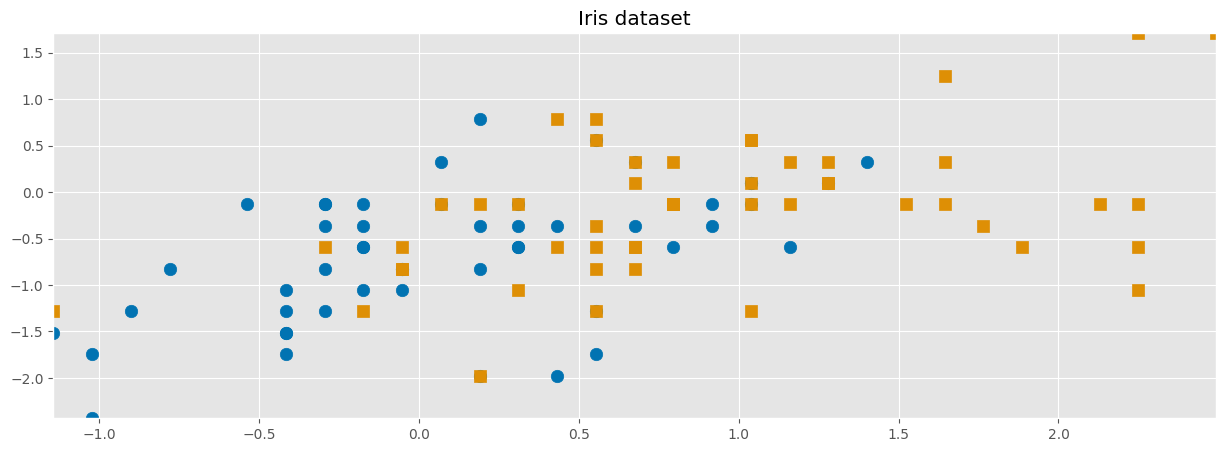
\includegraphics[width=\linewidth]{outputs/q1_dataset.png}
    \caption{Représentation de l'échantillon du dataset iris retenu.}
    \label{fig:iris_dataset}
\end{figure}

Nous allons à présent séparer notre jeu de données en deux afin de mettre des données de côté, caractérisant l'échantillon de test. Puis, en utilisant un noyau linéaire et à l'aide de la fonction \texttt{SVC} et  \texttt{GridSearchCV} (pour le choix des paramètres par validation croisée) de  \texttt{scikit-learn}. Nous obtenons une séparation que nous pouvons observer dans la Figure~\ref{fig:q1_CV}.
\begin{figure}[H]
    \centering
    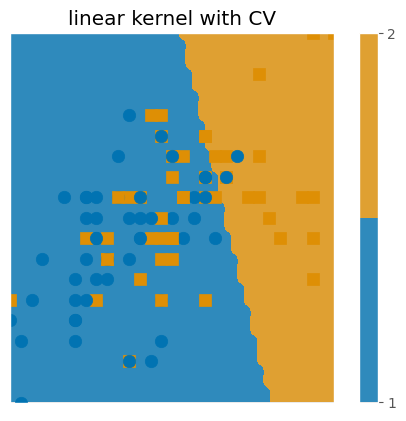
\includegraphics[width=.3\linewidth]{outputs/q1_with_CV.png}
    \caption{Représentation de la frontière du classifieur à noyau linéaire en utilisant la validation croisée}
    \label{fig:q1_CV}
\end{figure}
Nous calculons ensuite les scores de précision du modèle à noyau linéaire sur les données X et y, à la fois sur les données d'entraînement mais aussi et surtout sur les données de test. Il est à noter que ces scores peuvent dépendre d'une simulation à un autre.\\
En faisant une moyenne sur plusieurs simulations (30), nous obtenons un score sur les données d'apprentissage égal à $0.74$ et $0.6$ pour les données de test. Le score d'entraînement est plutôt bon, il représente la précision du modèle sur les données d'entraînement. Le score de test, ou score de généralisation, montre comment le modèle s'adapte à des données qu'il n'a pas vu auparavant (capacité de généralisation) . Les scores sont relativement proches, mais un score de test de $0.6$ peut soulever quelques préoccupations, notamment le fait que les données ne sont pas parfaitement linéaires, le modèle a du mal à séparer les données avec une simple droite affine. Cela implique que le modèle a besoins de certaines améliorations.

Nous faisons ensuite la même chose, mais cette fois sans utiliser la validation croisée, à l'aide de seulement la fonction \texttt{SVC} et un noyau linéaire. Nous obtenons un score moyen d'apprentissage égal à $0.74$, et un score de test égal à $0.68$. Nous observons la classification dans la Figure~\ref{fig:q1_noCV} suivante.
\begin{figure}[H]
    \centering
    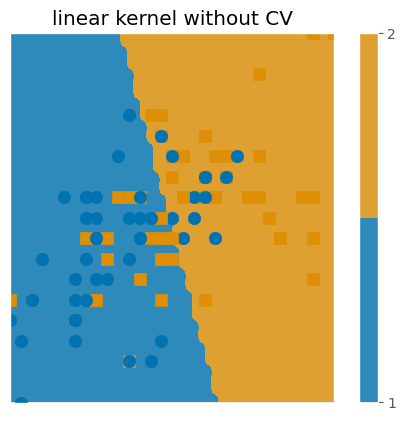
\includegraphics[width=.3\linewidth]{outputs/q1_without_CV.png}
    \caption{Représentation de la frontière du classifieur à noyau linéaire sans utiliser la validation croisée}
    \label{fig:q1_noCV}
\end{figure}

Il est à noter que sans validation croisée, le score de généralisation est en moyenne meilleur que lorsqu'on l'utilise. Le modèle a cependant toujours besoin d'améliorations si nous souhaitons avoir une généralisation satisfaisante et efficace.

\section{Question 2}

Nous allons essayer de trouver une amélioration, notamment en changeant le noyau. En effet, nous allons utiliser un noyau polynomial, puis comparer les scores avec ceux obtenus dans la question 1.\\
Après avoir calculé les scores d'entraînement et de test en faisant une moyenne sur 10 simulations (moindre à cause du temps de calcul), nous obtenons un score d'entraînement égal à $0.74$, ce qui n'a pas changé, et un score de généralisation égal à $0.68$, qui a lui augmenté. Pour le cas sans validation croisée, nous obtenons un score d'apprentissage moyen égal à $0.64$ et un score de généralisation égal à $0.62$.

\begin{figure}[H]
    \centering
\begin{subfigure}{0.45\linewidth}
    \centering
    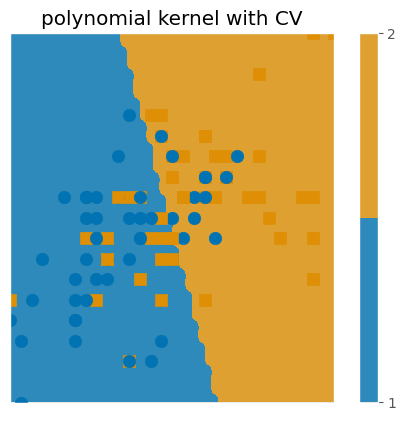
\includegraphics[width=0.5\linewidth]{outputs/q2_CV.png}
    \caption{Avec validation croisée}
    \label{fig:q2_CV}
\end{subfigure}
\begin{subfigure}{0.45\linewidth}
    \centering
    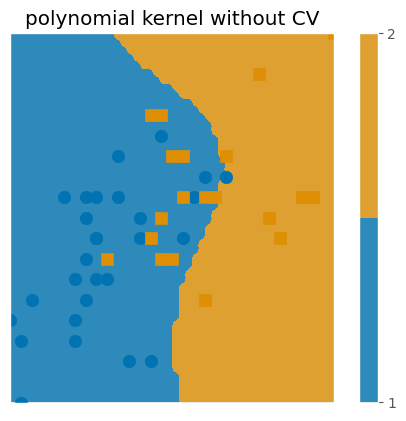
\includegraphics[width=0.5\linewidth]{outputs/q2_noCV.png}
    \caption{Sans validation croisée}
    \label{fig:q2_noCV}
\end{subfigure}
\caption{Représentation des deux frontières à noyau polynomial}

\end{figure}

Comme nous pouvons les voir dans les Figures~\ref{fig:q2_CV} et~\ref{fig:q2_noCV}, quand on n'utilise pas la validation croisée, nous observons bien une frontière avec une allure polynomiale.

Le fait que le score de généralisation augmente en changeant le noyau (kernel) (seulement avec l'utilisation de la validation croisée) signifie que le noyau polynomial permet au modèle de s'adapter d'une meilleure manière aux données étrangères que le noyau linéaire le lui permet. Cette légère augmentation de score signifie que les données contiennent certaines relations non-linéaires, mais celle-ci reste relative et ces relations ne semblent pas être très fortes. Quand nous ne l'utilisons pas, nous nous rendons compte que le modèle a toujours besoin d'améliorations.\\

\begin{figure}[H]
    \centering
    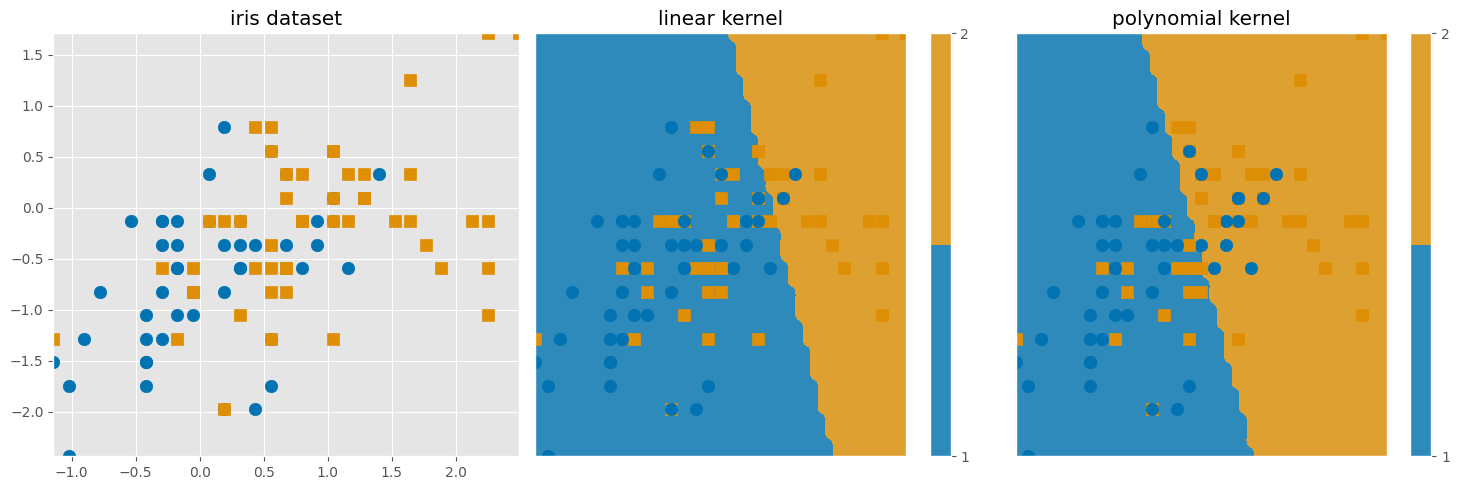
\includegraphics[width=.9\linewidth]{outputs/q2_compare.png}
    \caption{Comparaison des classifications selon les noyaux, avec validation croisée}
    \label{fig:q2_compare}
\end{figure}

Comme nous pouvons le voir sur la Figure~\ref{fig:q2_compare}, la différence de classification entre le noyau linéaire et polynomial n'est pas flagrante, tout comme les scores de généralisation. (Cela peut être dû au fait que pour le noyau polynomial, nous ajoutons des dimensions dans l'espace pour trouver un meilleur séparateur linéaire, puis pour des questions de visualisation, nous retournons en deux dimensions pour visualiser cette séparation.)

\begin{figure}[H]
    \centering
    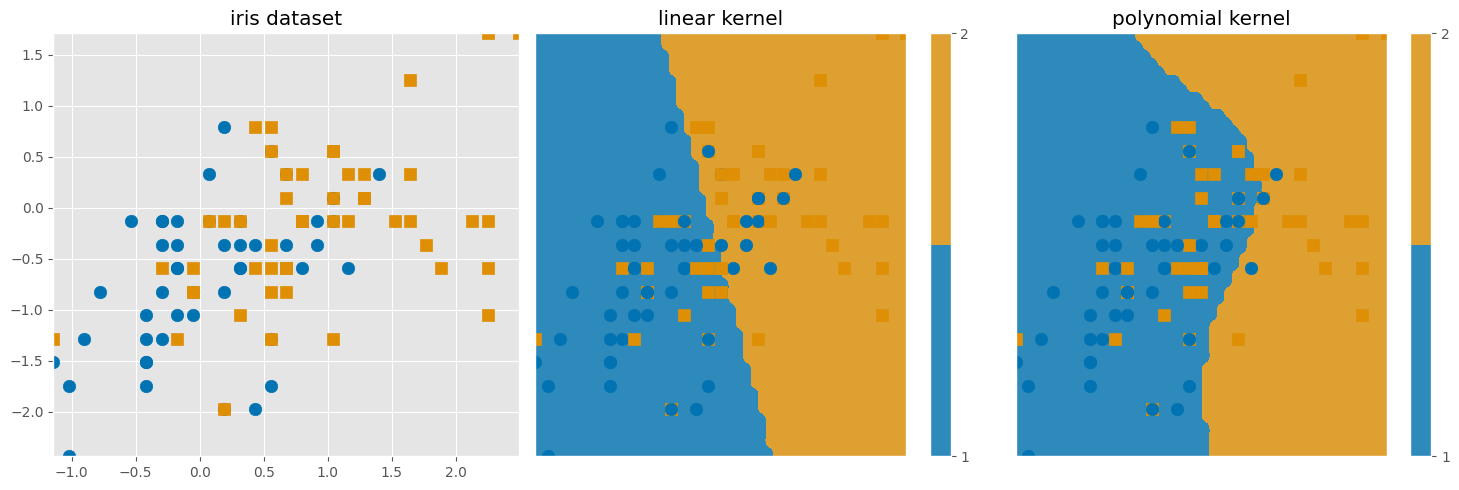
\includegraphics[width=.9\linewidth]{outputs/q2_compare_noCV.png}
    \caption{Comparaison des classifications selon les noyaux, sans validation croisée}
    \label{fig:q2_compare_noCV}
\end{figure}

Nous pouvons bien observer, dans la Figure~\ref{fig:q2_compare_noCV}, la différence de classification entre un noyau linéaire et un noyau polynomial. Cela est dû au fait que lorsque l'on n'utilise pas la validation croisée, la fonction \texttt{SVC} choisit automatiquement un degré égal à 3 pour le polynôme caractérisant le noyau.

\section{Question 3}
Nous allons utiliser une application interactive permettent de comprendre l'impact des différents paramètres des SVM. Pour cela, nous allons lancer le script \texttt{svm\_gui.py}, que l'on peut retrouver à l'adresse suivante : \url{https://scikit-learn.org/1.2/auto_examples/applications/svm_gui.html}, ou alors directement sur notre page Github, dans le dossier \texttt{src}.\\
Nous plaçons des points en les répartissant de manière à ce que le proportion de points d'une classe soit très supérieure à celle de l'autre. En faisant varier le paramètre $C$, de régularisation, nous obtenons les représentations suivantes.

\begin{figure}[H]
    \centering
    \captionsetup{justification=centering}
    % Première ligne : 2 images
    \begin{subfigure}{0.45\textwidth}
        \centering
        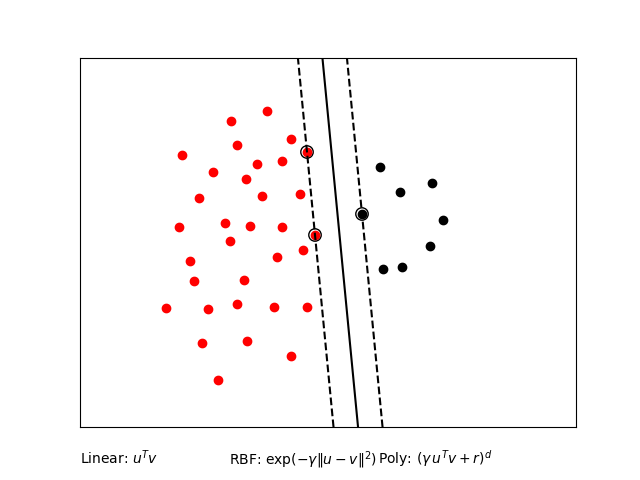
\includegraphics[width=.7\textwidth]{outputs/SVM_C_1.png} 
        \caption{Avec $C=1$}
    \end{subfigure}
    \begin{subfigure}{0.45\textwidth}
        \centering
        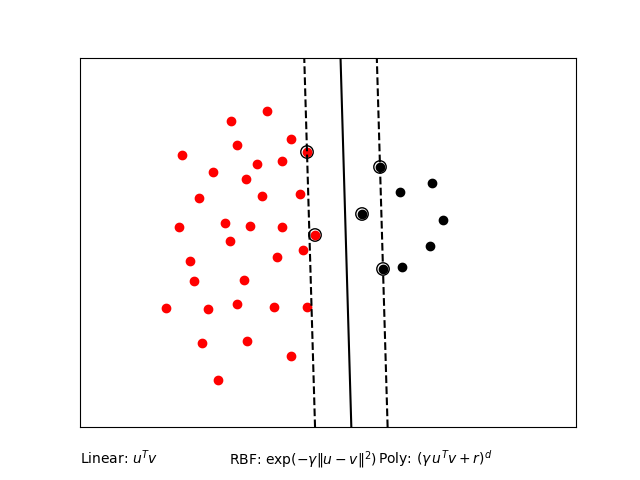
\includegraphics[width=.7\textwidth]{outputs/SVM_C_0_01.png}
        \caption{Avec $C=0.01$}

    \end{subfigure}

    \vspace{0cm} % Espace entre les deux rangées

    % Deuxième ligne : 2 images
    \begin{subfigure}{0.45\textwidth}
        \centering
        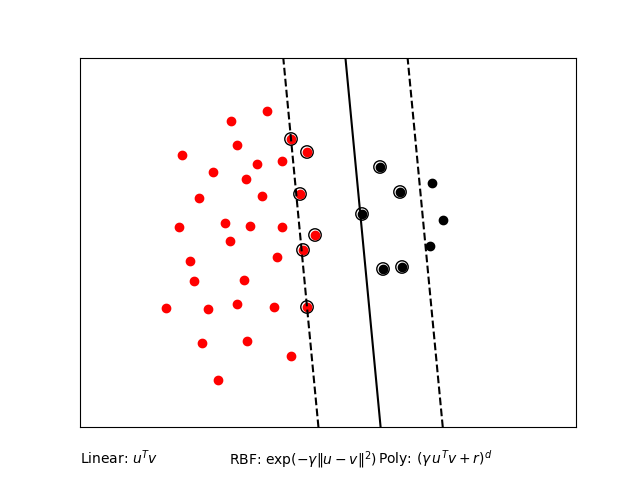
\includegraphics[width=.7\textwidth]{outputs/SVM_C_0_001.png} 
        \caption{Avec $C=0.001$}
    \end{subfigure}
    \begin{subfigure}{0.45\textwidth}
        \centering
        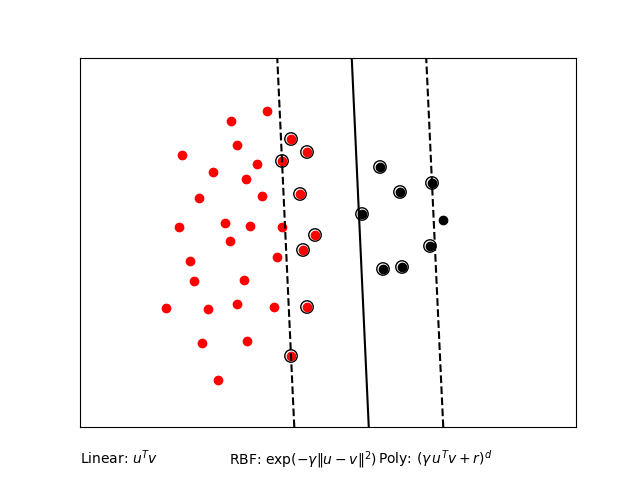
\includegraphics[width=.7\textwidth]{outputs/SVM_C_0_0005.png} 
        \caption{Avec $C=0.0005$}
    \end{subfigure}

    \caption{Représentation des différents résultats de classification en faisant varier le paramètre de régularisation C}
    \label{fig:q3_var_C}
\end{figure}

Comme nous pouvons le voir dans la Figure~\ref{fig:q3_var_C} ci-dessus, la variation de $C$ influe sur la taille de la fenêtre de séparation des classes, de taille $2\gamma$, où $\gamma$ est la marge maximale. Nous pouvons donc observer, pour toutes les valeurs de $C$, les différents vecteurs supports. $C$ étant le paramètre de régularisation de la marge souple, plus il est petit et plus le nombre de points entre les vecteurs supports ($\xi\in[0,1]$, avec $\xi$ une variable ressort), ou mal classés ($\xi>1$, pas présent dans notre exemple), est important.\\
De plus, plus la valeur de $C$ est faible, et plus le classifieur va dépendre de beaucoup de données, et donc le temps de calcul sera plus important, bien que les performances peuvent être améliorées.\\

Nous pouvons aussi remarquer que le classifieur ne prends pas en compte la proportion de données présentes dans chaque classe, omettant donc le poids de chaque nuage de points. Nous pouvons corriger ce phénomène en pondérant davantage les erreurs sur la classe la moins présente, ou alors par re-calibration.

\section{Question 4}

Nous allons à présent utiliser une banque d'images constituée de visages photographiés, nommée \textit{"Labeled Faces in the Wild"} (\url{http://vis-www.cs.umass.edu/lfw/}).

Parmi toutes les personnes présentes dans cette base de données, nous nous restreignons à deux personnées (variables) : Tony Blair et Colin Powell. Nous pouvons le voir sur la Figure~\ref{fig:q4_gallery} suivante.

\begin{figure}[H]
    \centering
    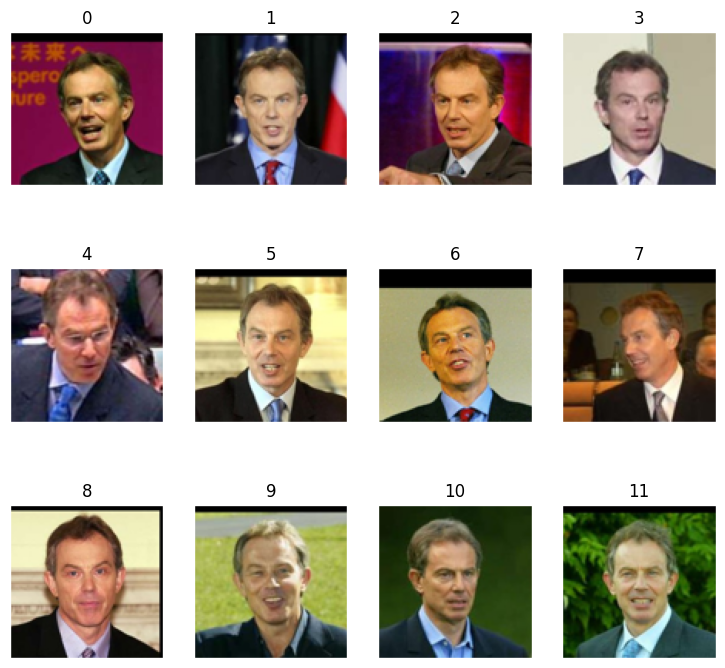
\includegraphics[width=0.35\linewidth]{outputs/q4_gallery.png}
    \caption{Exemple d'images présentes dans la base de données (Tony Blair)}
    \label{fig:q4_gallery}
\end{figure}

Dans cette question, nous allons chercher à montrer l'influence de ce paramètre de régularisation $C$. Pour cela, nous n'allons pas utilisé la validation croisée comme dans les deux premières question, mais simplement la fonction \texttt{SVC} du module \texttt{scikit-learn.svm} (si nous l'avions utilisé, nous aurions eu une droite constante). En faisant varier ce paramètre, nous allons chercher à retenir la meilleur valeur afin de prédire au mieux sur les données de test.

\begin{figure}[h]
    \centering
    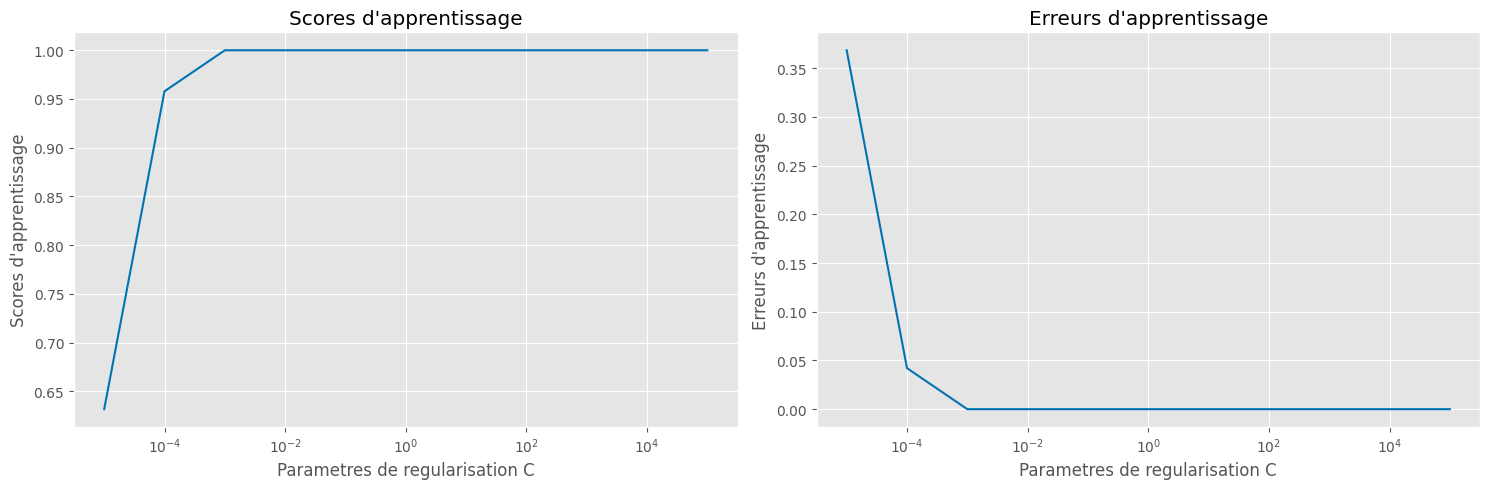
\includegraphics[width=.8\linewidth]{outputs/q4_scores_erreurs.png}
    \caption{Scores et erreurs d'apprentissage selon la valeur de $C$.}
    \label{fig:q4_score_erreur}
\end{figure}

Comme nous pouvons l'observer dans la Figure~\ref{fig:q4_score_erreur} ci-dessus, la meilleure valeur du paramètre $C$ de régularisation est $10¨{-3}$ puisque la valeur de score d'apprentissage est de $1$, et celle d'erreur d'apprentissage est de $0$.\\

Nous allons donc utiliser cette valeur pour recréer un classifieur linéaire, l'entraîner avec les données d'apprentissage, et le tester sur les données de test, en prédisant les valeurs $y$ de test à l'aide des valeurs $X$ de test et du modèle entraîné sur les données d'apprentissage.\\
Nous obtenons ainsi une précision de $0.9$, avec un niveau de chance (si le modèle ne fait rien de particulier pour apprendre ou généraliser, il se contente de prédire la classe majoritaire) de $0.62$. Nous avons donc une prédiction nettement meilleure que l'aléatoire, ce qui signifie que notre modèle a bien appris à classifier les données correctement ($90\%$ de précision).\\
\begin{figure}[H]
    \centering
    \captionsetup{justification=centering}
    % Première ligne : 2 images
    \begin{subfigure}{0.45\textwidth}
        \centering
        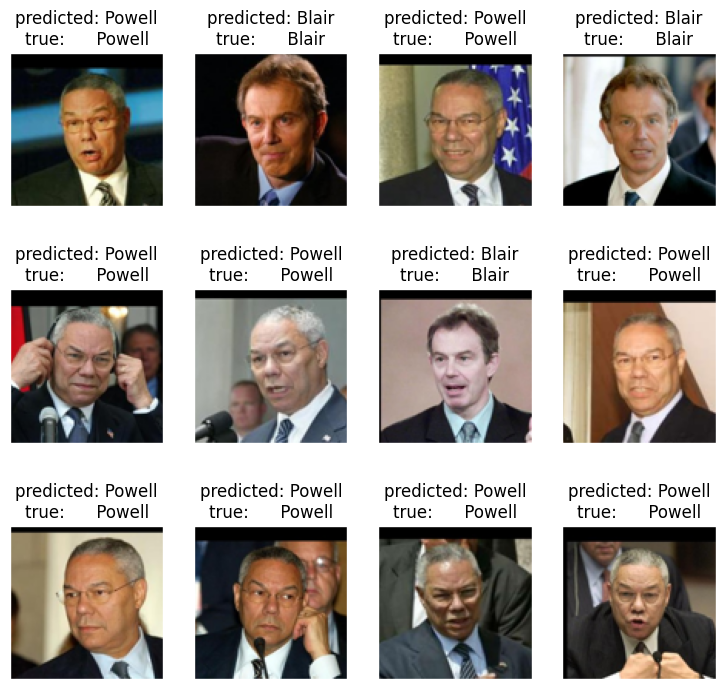
\includegraphics[width=.9\textwidth]{outputs/q4_prediction.png} 
        \caption{Prédictions}
        \label{fig:q4_prediction}
    \end{subfigure}
    \hfill
    \begin{subfigure}{0.45\textwidth}
        \centering
        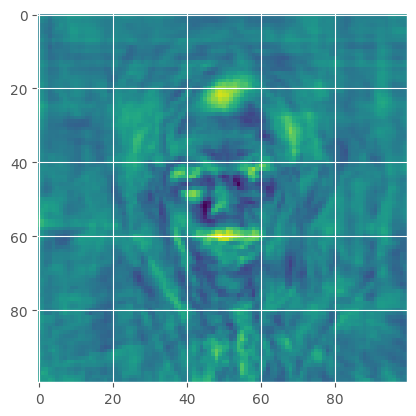
\includegraphics[width=.8\textwidth]{outputs/q4_coeffs.png}
        \caption{Coefficients}
        \label{fig:q4_coeffs}
    \end{subfigure}
    \caption{Représentation des prédiction et des coefficients de différenciation.}
\end{figure}

Nous pouvons donc vérifier si les prédictions sont vraiment précises à l'aide de la Figure~\ref{fig:q4_prediction}. Dans l'échantillon présenté, toutes les prédictions sont justes, mais il ne faut pas oublier qu'il y a une précision de $90\%$ avec ce classifieur.\\
De plus, nous pouvons aussi regarder une représentation des coefficients qui ont permis au classifieur d'atteindre une telle précision, dans la Figure~\ref{fig:q4_coeffs}. En effet, ce sont les zones en jaune qui ont le plus permis d'établir une différence entre les deux personnes que nous avons traitées. Le contour des yeux, de la bouche, et les cheveux semblent être les facteurs qui ont permis au classifieur de distinguer ces deux personnes.

\section{Question 5}

Nous allons à présent rajouter des variables de bruit dans notre modèle afin d'observer dans quelle mesure la performance de celui-ci est impactée. Tout d'abord, à l'aide de la fonction \texttt{run\_svm\_cv}, nous allons utiliser la validation croisée. Nous obtenons alors, sans ajouter de variables de nuisance, un score de généralisation (de test) égal à $0.9$ (moyenne sur 10 simulations). Lorsque l'on rajoute des variables de nuisance, nous obtenons un score de généralisation égal à $0.54$. La performance de notre modèle chute drastiquement.

\section{Question 6}

Nous pouvons améliorer cette prédiction à l'aide d'une réduction de dimensions en utilisant l'objet \\ \texttt{sklearn.decomposition.PCA(n\_components, svd\_solver='randomized')}. On remarque qu'en faisant varier la valeur de \texttt{n\_components}, le temps d'exécution peut changer du tout au tout. En effet, pour $n\_components = 100$, le code s'exécute en 1 seconde, mais quand on diminue la valeur de ce paramètre, le temps d'exécution augmente. Cela est dû au fait que ce paramètre représente le nombre de composantes que l'on souhaite garder après la réduction de dimension.\\
Pour $n\_components = 80$, nous trouvons un score de généralisation égal à $0.58$. Nous pouvons remarquer que l'amélioration reste relative, et qu'il faudrait baisser le nombre de dimensions à conserver pour augmenter ce score.


\end{document}
